\section{Graphical User Interface}
\label{sec:des_gui}

In the approach to creating a suitable interface for the graphs produced by the Hadoop cluster and due the nature of the projects design considerations, which in short is essentially a distributed system with an interface connected via simple object access protocol (SOAP) messages, a few extra design considerations were therefore given to the interface. As the GUI was a continuation of a previous years work, it was first necessary to analyse the structure of the interface, before any modification to the existing code. Another consideration of high importance was the suitability of the graphical visualizer for the graphs and how well the chosen libraries would cope with the size of graphs produced from the datasets we wished to use. A further problem which was analysed in the previous years work review earlier, exposed a complex dependency structure in which the the visualizer operates. This dependency structure lead to the creation of two possible design scenarios in the implementation of the GUI. One design scenario incorporates features of both the original SNAT project possibilities, along with the functionality of this project. 

\subsection{Challenges with continuation of previous project work}
A significant point to mention here is that, while most of the system created for this project is of an original nature, this interface to be used is a continuation of a previous project. This has therefore lead to some issues in modifying the code. Firstly, it was necessary to adjust ones working style to analyse and reverse-engineer the code already created, so that a fuller understand of the structure of the software could be obtained. Secondly, careful analysis of the previous years work had to be undertaken as essentially, our interface is to be developed from the existing tool, regardless of design approach taken. 

\subsection{Graphical User Interface Design Objectives}
As the interface is only one part of a much larger system, it was first necessary to generate some design objectives. This stage is an important consideration when modifying an existing piece of software. Removal or addition of modules or a conflicting of modules could result in the interface becoming non-functional for simply trivial reasons. These "simple" errors can result in massive delays to the implementation process as re-checking of functional base code is necessary to determine whether or not an error is due to a design fault or issue with the previous groups work. Therefore to ensure that the interface was constructed with a reasonable focus in mind on the main objectives of the project, the following design objectives were given to the interface. These objectives were designed to allow the interface: 

\begin{itemize}
	\item To allow suitable connection to the hadoop cluster through use of SOAP messages
	
	\item To connect to the hadoop cluster and perform operations on the cluster such as:
	\begin{itemize}
		\item Upload Algorithms
		\item Upload Dataset
		\item Get Algorithms
		\item Get Dataset
		\item Execute Algorithm
		\item Get Results
		\item Show Statistics
	\end{itemize}
	
	\item To maintain the look and feel of the original interface
	
	\item To follow either one of the two design considerations
\end{itemize}

Therefore the extra objectives for the design of the interface were to:
\begin{itemize}
	\item Remove and insert web-service code into the existing software, while removing any excess code which could cause performance issues
	
	\item Analyse and scale the performance of test data on the visualiser
	
	\item Ensure that the database scheme is reverse-engineered correctly via testing through the visualiser.
	
	\item Ensure that the GUI is suitable to the overall outcome of the project
\end{itemize}

\subsection{The Existing Design}
We shall view the existing SNAT project with regards to only the current projects requirements in terms of the visualisation and GUI. The interface was developed using Microsoft Visual Studio 2010 with the C\# .net framework for the reason that the interface would become simpler to design and construct as the IDE has code completion and management functions. While this module management system is fantastic for developing, in terms of dissecting the code and locating key variables and other important constructs, it was in fact a very troublesome feature. Another issue, was with the compatibility of the IDE with SOAP library's built for C\#, and the lack of them too, however, we shall examine that later.


The first step is to analyse the dependency structure of the GUI in the SNAT project. 

The dependency structure of the GUI starting with the GUI is as show in Table \ref{tab:guidep}.

\begin{table}[htbp]%
\centering
\begin{tabular}{|l|l|}
\hline
Module & Dependency \\
\hline
GUI	& Network Model, Algorithms API \\
Algorithms API	& Network Model, Database Proxy \\
Network Model	& Database Proxy \\
Database Proxy	& Database \\
Database	& ***No dependencies*** \\
\hline
\end{tabular}
\caption{Dependency of GUI on other SNAT project components}
\label{tab:guidep}
\end{table}

The GUI is heavily dependant on nearly every other module from the previous SNAT project. Each main module is also made up of much smaller submodules which means that in terms of converting the existing interface into a suitable GUI for the distributed SNAT project, a full examination of the previous tools code was required, a very large task. 

Sticking with just the dependency structure of the SNAT code, it was clear that there are two possible designs that could be utilized. The reason for this is because the dependency of certain modules can be offloaded onto the cluster, however, this route should be avoided given the delayed start, as the complexity is dramatically greater than that of the simple implementation which is specified below.

\subsection{GUI Design}

\subsubsection{Design 1}
Dual-function: Combination of SNAT and DSNAT software linked via SOAP messages

The principle behind this design frame of the distributed social network analysis tool's interface is the simplicity in which the goal could be achieved via the use of SOAP messages inserted in key locations, whereby, a web-service would perform the function that the local version would do within the currently available SNA tool. Essentially the process would involve the following as illustrated in Figure \ref{fig:des1}

\begin{figure}[htbp]%
\centering
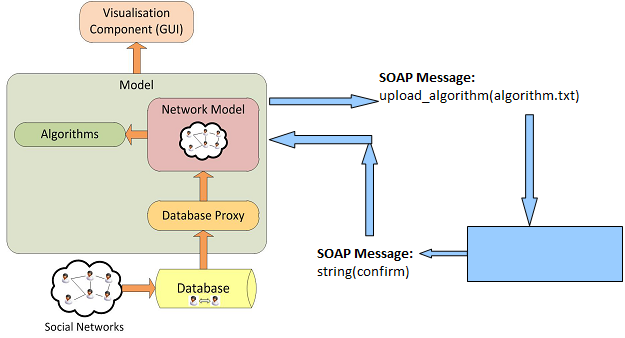
\includegraphics[width=0.6\columnwidth]{./img/des1}%
\caption{Insertion of SOAP messages into current system}%
\label{fig:des1}%
\end{figure}

Code would need to be strategically removed from the existing code to ensure that the visualiser and GUI only view one set of data and system variables at any one time. The overall design we shall not go into much detail, as it is quite simple. The overall code structure of the system would remain the same, however, methods that would have been called on the local software, would instead call a web-service, which should send a SOAP message, detailing the action of the cluster. The data would be processed through the cluster, with results being uploaded to the database, whereby the visualiser should play through the tape produced with statistics either being derived from the data locally, or remotely via another SOAP message communication with the cluster.

Advantages of this design:
\begin{itemize}
	\item Allows for minimal changes to existing code which should provide an easier platform in which debugging can take place
	
	\item Simple addition of a switch could alter connection state with server, e.g. implementation of an offline mode where a local SQL database could be connected
	
	\item Minimal reliance on cluster to process visualisation
	
	\item Safer option than design \#2 with respect to time constant
\end{itemize}

Disadvantages of this desgin:
\begin{itemize}
	\item Visualisation heavily dependent on specification of local system
	
	\item Database handling conducted by local machine
	
	\item Current software may not be compatible in terms of design to incorporate SOAP functionality, however, this is due to the dependencies associated with the rest of the system. Careful consideration of each methods responsibilities and actions should prevent this becoming a problem
\end{itemize}

One disadvantage noted above, is that the visualiser is heavily dependent on the specification of the machine on which the software is locally running on. The main concern with this issue is that, with the size of graphs this project is aiming to achieve in terms of long run goals, a situation where the visualisers performance could be subject to question, is extremely likely. However, testing of the interface with increasing magnitudes of datasets should determine whether or not the current interface visualisation techniques are suitable to this project.

\subsubsection{Design 2}
The second design is radically different from the first, however still manages to incorporate the features and feel of the original interface. As opposed to the design details above, the GUI would work in the following manner. 

The network view model and all functionality stripped from the GUI module and dependency cut. The network model and algorithms modules would move onto the cluster where the graph would be generated. However, this design obviously has some flaws, which is mostly due to the complexity. Figure \ref{fig:des2} represents the system dataflow design.

\begin{figure}[htbp]%
\centering
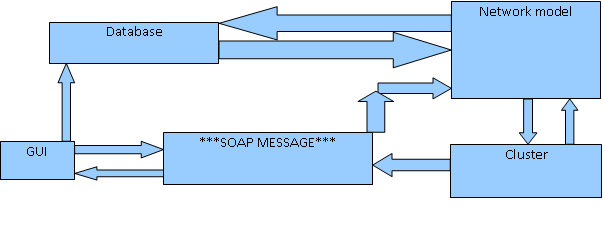
\includegraphics[width=0.6\columnwidth]{./img/des2}%
\caption{Design overview of standalone visualiser client with cluster processed imaging}%
\label{fig:des2}%
\end{figure}

The GUI is the only running module that exists from the SNAT project, with the network view model associated with the cluster rather than the interface. However, this design will not be used for a few simple reasons:

\begin{itemize}
	\item The design is far too complex. This design would require complete re-working of the current network view model and also the cluster design to incorporate the generation of the network view model
	
	\item This design does not alleviate any concerns regarding the current visualiser. As the method of graph visualisation is through the plug-ins GraphSharp and QuickGraph, the visualisation power is only as strong as the system running the plug-ins
	
	\item The cluster will be run on the Linux operating system, which therefore means conversion of or possible running of the code within mono, which is not suitable with some components of the system.
\end{itemize}

An alternative to the current visualiser, is the possible use of cytoscape, an open source network analysis tool. However, this visualisation technique will only be considered depending on the performance testing of the current visualiser.

\subsection{Visual Studio}
The chosen development environment for the DSNAT's GUI was Microsoft Visual Studio 2010 with the C\# .net environment. Essentially the same IDE was used and a copy of the project at that point in time, secured from the previous groups website at \url{http://code.google.com/p/snat/source/browse/trunk/snat/snat/snat.csproj} where the file located at this point would allow an import of the Visual Studio solution.

While the IDE chosen, allowed for quicker analysis of the current project code as it made it easier to follow the reports and guides that were written by the previous group, it had a drawback, as alteration to code generated by other is always a complex and tiresome task, resulting in errors usually caused by misunderstanding of the currently implemented code, further hindered by the complex and the wizard creation style of web-service generation that visual studio provides.

To gain a further understanding of the web-services that can be developed within visual studio, below is an example of a web-service being generated within Microsoft Visual Studio.

\subsubsection{Web-service generation in Visual Studio}

Pre-requisites:
\begin{itemize}
	\item Internet-information services needs to be running in order for the WSDL to work correctly.
	
	\item Microsoft Visual Studio 2010
\end{itemize}

\subsubsection{Adding a web-service client application in Microsoft Visual Studio 2010}
The first step in creating a web-service in Visual Studio 2010 is to ensure that  the virtual directory and name of the SOAP type is created. As each SOAP type has a web service definition language (WSDL) file associated with it, this is the location in which each method call will be stored and all procedures relating to the functioning of the web-service interface defined. 
Therefore before anything else we must first add a web reference to the project and specify the URL to the virtual name of SOAP type, followed by ``?wsdl''. 

Visual Studio then creates a Web service proxy class and adds it to the project. This proxy class details the methods of the web-service (defined by the WSDL file). By using this proxy class, any of the methods exposed by the virtual name can be invoked. After each request the server sends to the client in the format that was specified for that method during configuration of the virtual name of soap type the data or action requested.

The result of an operation can be returned  as one of the following types: 
\begin{itemize}
	\item XMLElement (System.Xml.XmlElement) or DataSet (System.Data.DataSet) type array 
	
	\item SqlMessage type array elements, which holds error messages that are returned
	
	\item SqlResultCode type array elements, which holds the return value when a UDF that returns a table or a stored procedure is executed 
\end{itemize}

The main data types of the SOAP interface that we shall be using, will be the XMLElement element.

Limitation of using Visual Studio when adding a SOAP reference is that the methods of incorporating the web-service is completely dependent on the style that Microsoft designed for Visual-studio. Another issue is that the insertion of a web-service is extremely complex when compared to that of another library such as Axis Apache 2. 
